\section{Discussion}\label{sec:disc}

\begin{figure}
\centering
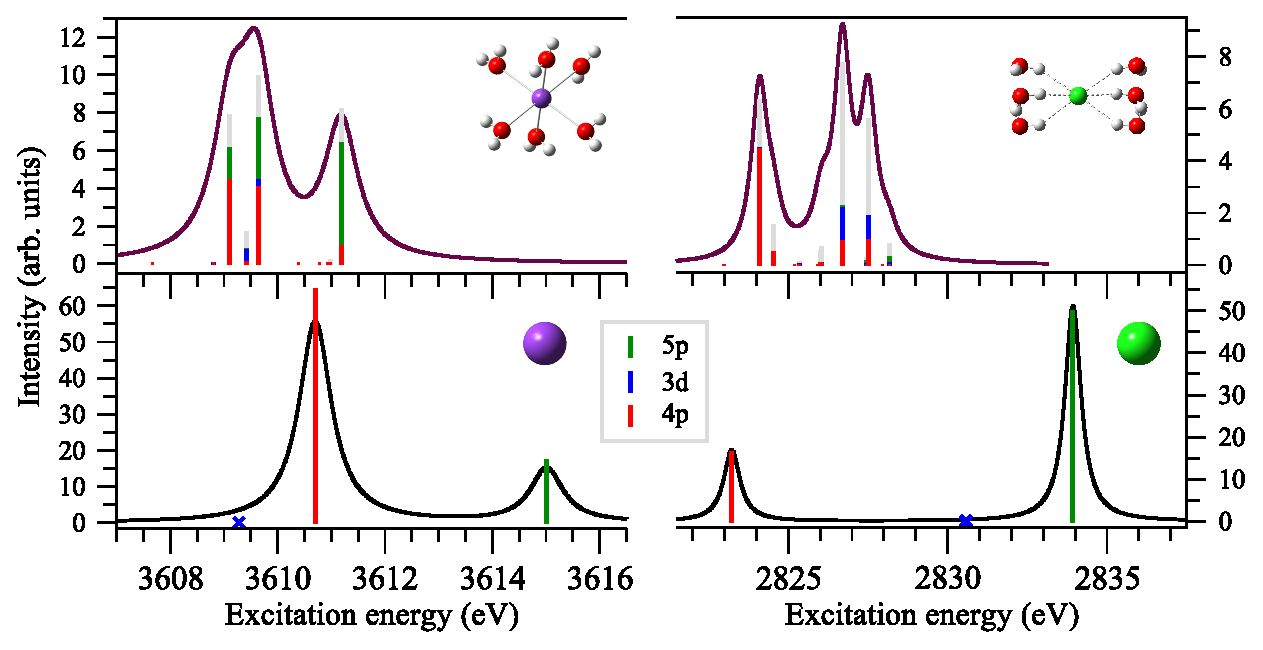
\includegraphics[scale=0.6]{figures/xas_spectra.eps}
\caption{
XAS spectra of the lowest K-shell transitions in the bare K$^{+}$ (lower left panel) and Cl$^{-}$ (lower right panel) ions and their 6-coordinated clusters (upper left panel, \ki(H$_2$O)$_6$, and upper right panel, \cli(H$_2$O)$_6$). The theoretical stick spectra were convolved with a Lorentzian profile of FWHM 0.74\,eV for \ki~and 0.62\,eV for \cli~in order to account for the lifetime broadening. The stick spectrum corresponds to the projections $|a_{nl}^{i}|^2$ of the SONOs corresponding to the core excited states of the 6-coordinated clusters on the basis of SONOs corresponding to the 1s$\,\rightarrow\,$3d, 1s$\,\rightarrow\,$4p, and 1s$\,\rightarrow\,$5p states in the bare K$^+$ and \cli~ions (Eq.\ \ref{eq:sono_proj}). The theoretical XAS spectra of \ki~were shifted to higher photon energies by 6.7\,eV, which corresponds to the difference between the computed and experimental core excitation energies of the 1s $\rightarrow$ 4p excitation in the bare ion taken from Ref.\ \citep{hertlein06:062715}.}
\label{fg:xas_kcl}
\end{figure}


In order to understand the resonant Auger features in the experimental AES spectra we computed the X-ray absorption spectra of both \ki~and \cli~and their microsolvated clusters with 1, 2, 4 and 6 water molecules, as well as the final Auger states of the bare ions.


The theoretical XAS spectra are presented in Figs.\ \ref{fg:xas_kcl} and \ref{fg:xas_kcl}. For both \ki~and \cli~(lowermost panels), the first observed peak in the XAS spectrum corresponds to the 1s$\,\rightarrow\,$4p state. It is noteworthy that the positions of the 1s$\,\rightarrow\,$4p and 1s$\,\rightarrow\,$3d states are inverted in \ki~and \cli. In the case of Cl$^{-}$ the 1s$\,\rightarrow\,$4p excitation has lower energy and the 1s$\,\rightarrow\,$3d excitation is close to the 1s$\,\rightarrow\,$5p state. On the contrary, in K$^{+}$ the 1s$\,\rightarrow\,$3d excitation has lower energy and lies below the 1s$\,\rightarrow\,$4p state. It is noteworthy that the intensity of the 1s$\,\rightarrow\,$4p state is lower than that of the 1s$\,\rightarrow\,$5p state in \cli. An explanation of this phenomenon can be found in the Supporting Information.


%1.4 Solvated clusters:

In what follows, we will focus on the fate of the lowest-lying peak in the XAS spectra of \ki~and \cli, originating from the excitation of a 1s electron to the 4p unoccupied orbital (Figs.\ \ref{fg:xas_kcl} and \ref{fg:xas_kcl}). In the case of \ki~the position of the peak drops from 3610.7\,eV in the bare ion \citep{hertlein06:062715} to 3608.7\,eV in the 4-coordinated cluster, whereas in the case of \cli~the solvent molecules have little influence on the position of the first peak (it varies between 2823.3\,eV for the ion and 2824.2\,eV for the 6-coordinated cluster). Since the peak is broadened due to the finite lifetime and the splitting of the core excited states in the ligand field of the solvent, and because the 1s ionization potential of \ki~drops by $\sim$7\,eV in a solution \citep{ceolin17} compared to the bare ion \citep{hertlein06:062715}, which is more than the difference between the 1s$\,\rightarrow\,$4p and 1s$\,\rightarrow\,$5p states, we expect that these states are the only states populated below the ionization threshold.


Let us first consider how the 1s$\,\rightarrow\,$4p core excitation of \ki~is influenced by the presence of the solvent (see Fig.\ \ref{fg:xas_kcl}). In the singly- and doubly-coordinated clusters, the 1s$\,\rightarrow\,$4p excitation splits into groups of states, which results in the formation of a low-intensity shoulder on the high photon energy side of the main peak in the theoretical XAS spectra. The situation is substantially different for the 4-coordinated clusters, where the first peak in the XAS spectrum is produced by states with a small contribution from the dipole allowed 1s$\,\rightarrow\,$4p state and a large contribution $\sim$40\% from the dark 1s$\,\rightarrow\,$3d states. The latter states acquire intensity due to mixing with the 4p-states in the ligand field created by the solvent. A similar effect was observed in the microsolvated clusters of Na$^{+}$ and Mg$^{2+}$ \citep{miteva16:16671}. Finally, in the 6-coordinated cluster, which represents the complete first solvation shell around \ki, the lowest peak in the spectrum contains the 1s$\,\rightarrow\,$4p states split by approximately 0.5\,eV, and a low intensity state in between, which has a predominantly 1s$\,\rightarrow\,$3d character, and which also acquires intensity due to mixing with the bright 4p- and 5p-core excited states.


In the case of \cli, the water molecules tend to gather on one side of the \cli~ion and form H-bonds with it \citep{ge13:13169}. The resulting structures are of lower symmetry compared to the respective microsolvated clusters of \ki, which influences the splitting of the states of the bare ion upon the addition of solvent molecules (Fig.\ \ref{fg:xas_kcl}). This effect is most pronounced for the higher lying 1s$\,\rightarrow\,$5p states and it does not substantially. The lowest lying 1s$\,\rightarrow\,$4p excitation in \cli~can still be identified in the microsolvated clusters. Moreover, this state does not interact strongly with the 1s$\,\rightarrow\,$3d state because as earlier discussed, they do not lie close in energy in the bare ion.


\begin{figure}[h!]
\centering
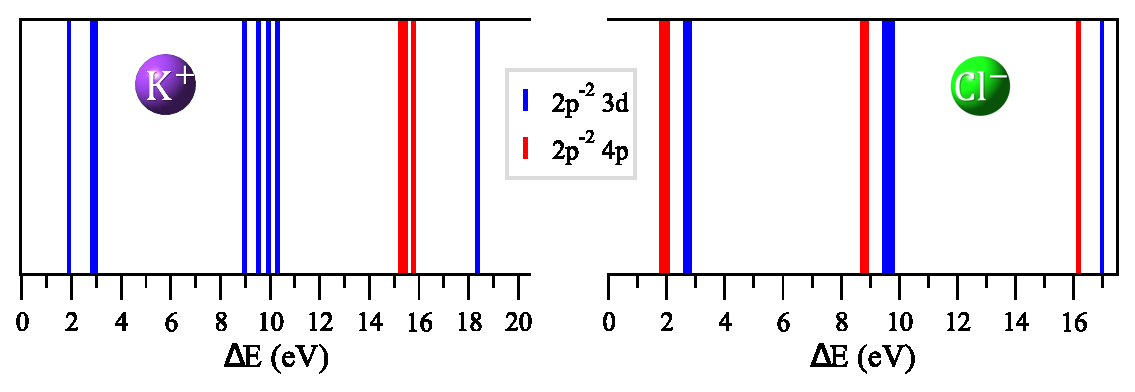
\includegraphics[scale=0.6]{figures/kcl_2p-2nl.eps}
\caption{Final 2p$^{-2}$($^3$P, $^1$D) 3d, 4s, 4p doublet Auger states of K$^{+}$ (left) and Cl$^{-}$ (right) computed at the CIS level (see Sec.\ \ref{sec:methods} for details). The states are shifted with respect to the lowest quartet state with electron configuration 2p$^{-2}$($^3$P) 4s.}
\label{fg:kcl_2p4nl}
\end{figure}


Solely from the XAS spectra, one cannot extract information about the course of the subsequent Auger process. As can be seen on the 2D maps of \ki~and \cli, the resonant Auger process is the decay pathway of the lowest lying core excited states. In what follows, we attempt to explain the dispersive features in the experimental spectra of \ki~and \cli,~and understand the interrelation between the electronic structure of the core excited species and their Auger electron spectra. To this end we computed the lowest K$^{2+}$(2p$^{-2}$nl) and Cl$^{0}$(2p$^{-2}$nl) states corresponding to the lowest final spectator resonant Auger states (Fig.\ \ref{fg:kcl_2p4nl}). Out of all final states we discuss only the doublets assuming that the quartet states are populated with a very low probability (REFS). Already at the level of the bare ion one can see that the 2p$^{-2}$nl states of \ki~and \cli~are substantially different. They reflect the fact that the 3d unoccupied orbitals of \ki~are lower than the 4p orbitals, which is the opposite of what is observed in \cli.


The lowest doublet states of \ki~are the 2p$^{-2}$3d states, they form two groups of states around 2\,eV and 10\,eV above the lowest quartet state. The lowest 2p$^{-2}$4p states, on their turn, appear between 15 and 16\,eV, and are thus well separated in energy from the 2p$^{-2}$3d states. In the resonant Auger decay the lowest 4p-states which can be populated, are therefore those located between 15 and 16\,eV above the lowest quartet state. Consequently, we can assume that resonant Auger decay of the lowest core-excited states of \ki~which have a mixed 1s$\,\rightarrow\,$4p/5p character leads to the population of these states and thus to the formation of the dispersive feature B on Fig.\ \ref{fg:2dmap_k}. The second dispersive feature, C, appears at higher kinetic energies of the Auger electron and, consequently, it will result from the population of lower lying spectator Auger states. The lower-lying states in the K$^{2+}$(2p$^{-2}$nl) spectrum are of 2p$^{-2}$3d character. These states can be populated as a result of the resonant Auger decay of the dipole forbidden 1s$\,\rightarrow\,$3d states which acquire intensity in the 4- and 6-coordinated clusters due to mixing with dipole allowed 4p-states in the presence of the solvent. The splitting between the maxima of B and C is $\sim$400\,meV, which coincides with the splitting between the first 1s$\,\rightarrow\,$4p and the 1s$\,\rightarrow\,$3d excitations in the theoretical spectrum of the 6-coordinated cluster (Fig.\ \ref{fg:xas_kcl}). Moreover, in the theoretical spectrum the intensity of the 1s$\,\rightarrow\,$3d state is much lower than that of the 1s$\,\rightarrow\,$4p states. Consequently, the fingerprint of the former state in the Auger electron spectrum will be of lower intensity compared to the latter one. This is in compliance with the experimentally observed lower intensity of island C compared to island B (see Fig.\ \ref{fg:intensity_ratio}). Therefore, we can conclude that the island C on Fig.\ \ref{fg:2dmap_k} is a result of the resonant Auger decay of the dipole forbidden 3d-core excited state of the hydrated \ki~ion, whereas the dispersive feature B is a result of spectator resonant Auger decay of states of predominantly 1s$\,\rightarrow\,$4p character.


In the Cl$^{0}$(2p$^{-2}$nl) spectrum there are two groups of states split by about 7\,eV. These two groups of states are energetically separated not by the virtual orbital occupied by the excited electron, but rather by the configuration of the two holes. As can be seen in Fig.\ \ref{fg:kcl_2p4nl}, there are the 2p$^{-2}$($^3$P)4p,3d and 2p$^{-2}$($^1$D)4p,3d states located around 2 and 9\,eV, respectively. Consequently, even if the initial core-excited states of aqueous \cli~are mixed 1s$\,\rightarrow\,$3d and 1s$\,\rightarrow\,$4p states of the bare ion, one will not observe separate dispersive features from spectator resonant Auger to the 2p$^{-2}$3d and 4p final states.

%
%
%The formation of such an island on the 2D map of \ki$_{\text{aq}}$ can result from several processes: shake-up resonant Auger decay, similar to the case of Ar \citep{ceolin15:022502}, spin-orbit splitting in the final states, core-like ICD process, or population of dipole forbidden states, which is a result of symmetry breaking in the presence of the solvent. 
%
%\begin{enumerate}
%
%\item[a)] Shake-up resonant Auger decay
%
%A separate island at 2666\,eV kinetic energy and 3203.5\,eV photon energy is observed on the 2D map of Ar (see Fig.\ 2 in \citep{ceolin15:022502}. This island results from resonant Auger decay of the Ar 1s$\,\rightarrow\,$4p state to Ar$^{2+}$(2p$^{-2}$4p) states. The 1s$\,\rightarrow\,$4p state undergoes also shake-up resonant Auger decay, resulting in the population of Ar$^{2+}$(2p$^{-2}$5p) states which appear as a separate feature at the same photon energy, but at lower kinetic energies, 2662\,eV.
%
%
%A similar shake-up decay can be expected for the 1s$\,\rightarrow\,$4p state of \ki. As a first step, we estimate the splitting between the 2p$^{-2}$4p and 2p$^{-2}$5p final states. Using the $(Z+2)$-approximation, the splitting between the 2p$^{-2}$4p and 2p$^{-2}$5p states of K$^{3+}$ is equal to the splitting between the 3p$^6$4p and 3p$^6$5p states of Sc$^{3+}$. From the NIST database \citep{NIST_ASD} for the bare ion we obtain $\sim$8.2\,eV, which agrees with the splitting between the island and the dispersive feature close to the $^1$D main line on the 2D map of \ki$_\text{aq}$ (Fig.\ \ref{fg:2dmap_k}). As a second step, we compare the intensity ratio between the two dispersive features in \ki$_{\text{aq}}$ with that in Ar. As can be seen from Fig.\ \ref{fg:intensity_ratio} the lower-lying peak, which is attributed to the K$^{3+}$(2p$^{-2}$5p) state has higher intensity compared to the higher-lying peak. The intensity of the two peaks in Ar is exactly the opposite implying a lower shake-up probability. Another counterargument against the shake-up origin of the island is that if one compares the maxima of the two dispersive features B and C, one sees that the feature B appears at lower photon energies than C. This is opposed to Ar, where the island originating from normal Auger decay appears at lower photon energies.
%
%Another question is whether the 2p$^{-2}$5p states can be populated in a solution. To address this issue, on Fig.\ \ref{fg:k_2p4nl_raddens} we compare the radial density distributions of the natural orbitals occupied by the excited electron in the K$^{3+}$(2p$^{-2}$4p) and K$^{3+}$(2p$^{-2}$5p) states. The former distribution is quite compact, with 86\% of the electron density within the first solvation shell, whereas only about 20\% of the electron density in the  K$^{3+}$(2p$^{-2}$5p) state is within the first solvation shell.
%
%
%Therefore, we conclude that the features B and C on the 2D map of \ki$_{\text{aq}}$ Fig.\ \ref{fg:2dmap_k} are not a result of a shake-up and normal Auger decay of the \ki(1s$\,\rightarrow\,$4p) state.
%
%\end{enumerate}
%
%
%{\color{blue}\bf Discuss the possibility for non-local Auger decay! Spin-orbit splitting of the final states: it cannot give such a big difference (of 8\,eV)}